\section{Alignment Regimes}
\label{sec:regimes}

The spectrum of the alignment operator $H = G^{-1}C$ naturally partitions the
behavior of empirical sensitivity into three fundamental regimes:
\emph{equilibrium}, \emph{sup\-pression}, and \emph{excess alignment}. Each regime
corresponds to a distinct empirical deformation of Fisher--Rao geometry and has
clear geometric and statistical interpretation.

We summarize these regimes below before turning to empirical demonstrations.

\begin{figure}[t]
\centering

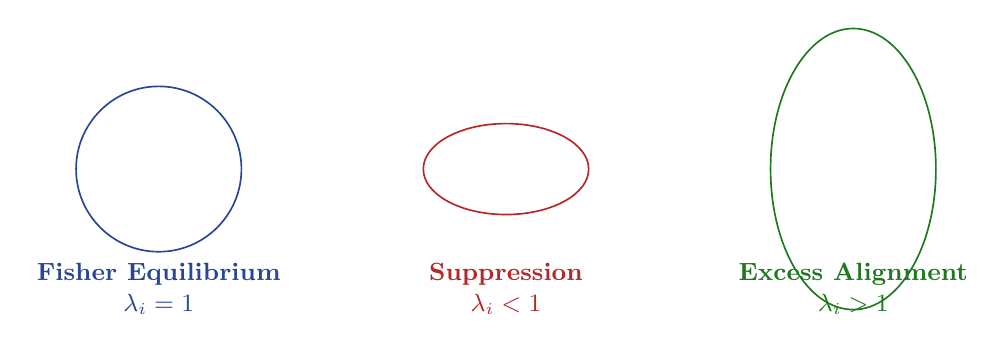
\begin{tikzpicture}[scale=1.05]

    % Colors in a more professional physics palette
    \definecolor{eqcol}{RGB}{40,70,150}
    \definecolor{supcol}{RGB}{180,40,40}
    \definecolor{excol}{RGB}{30,120,30}

    % Common text style
    \tikzset{
        reglabel/.style={font=\small\bfseries, align=center}
    }

    % ============== Fisher equilibrium (circle) ==============
    \begin{scope}[xshift=0cm]
        \draw[semithick, eqcol] (0,0) circle (1cm);
        \node[eqcol, reglabel] at (0,-1.45)
            {Fisher Equilibrium\\$\lambda_i = 1$};
    \end{scope}

    % ================== Suppression ellipse ==================
    \begin{scope}[xshift=4.2cm]
        \draw[semithick, supcol] (0,0) ellipse (1cm and 0.55cm);
        \node[supcol, reglabel] at (0,-1.45)
            {Suppression\\$\lambda_i < 1$};
    \end{scope}

    % ================= Excess Alignment ellipse ==============
    \begin{scope}[xshift=8.4cm]
        \draw[semithick, excol] (0,0) ellipse (1cm and 1.7cm);
        \node[excol, reglabel] at (0,-1.45)
            {Excess Alignment\\$\lambda_i > 1$};
    \end{scope}

\end{tikzpicture}

\caption{
Geometric regimes of empirical alignment on a Fisher manifold.
Equilibrium corresponds to isotropic curvature ($\lambda_i=1$),
suppression reflects contraction of sensitivity along one or more axes
($\lambda_i<1$), and excess alignment corresponds to expansion beyond
the Fisher baseline ($\lambda_i>1$).
}
\label{fig:alignment-regimes}
\end{figure}


% -------------------------------------------------------------
\subsection{Fisher Equilibrium}

A model is in Fisher equilibrium at $\theta$ when
\[
\lambda_i(\theta;q) = 1 \quad \text{for all } i.
\]
In this regime, empirical score covariance matches the geometric expectation set
by the Fisher metric. The alignment tensor vanishes,
\[
\Delta_{ij} = 0,
\qquad
\mathcal{A} = 0,
\qquad
\phi = 0,
\]
and the empirical sensitivity landscape is isotropic in Fisher-orthonormal
coordinates.

This regime occurs when $q=p$ in minimal exponential families
\cite{Brown1986,WainwrightJordan2008} or when empirical and model curvature
coincide despite mild model misspecification. Gaussian families (with mean and
variance parameters) provide canonical examples.

% -------------------------------------------------------------
\subsection{Suppression Regime}

The suppression regime corresponds to
\[
\lambda_i < 1 \quad \text{for one or more eigenvalues}.
\]
Here empirical variance falls \emph{below} the Fisher--Rao baseline, indicating
that the data distribution $q$ concentrates sensitivity into a lower-dimensional
tangent subspace than predicted by the model.

Key signatures:
\[
\mathcal{A} < 0,
\qquad
\phi = 0,
\]
reflecting a net contraction of empirical sensitivity.

Suppression manifests in models with heavy-tailed likelihood structure, sharp
modes, or symmetry-induced collapse. The Laplace family provides a simple
example: even under $q=p$, empirical curvature does not match Fisher curvature,
yielding slight suppression \cite{LaplaceDistribution}.

Geometrically, suppression corresponds to a flattening of the empirical local
quadratic structure relative to the intrinsic Fisher geometry.

% -------------------------------------------------------------
\subsection{Excess Alignment}

Excess alignment occurs when
\[
\exists\, i : \lambda_i > 1,
\]
and is characterized by empirical reinforcement along one or more
Fisher-orthonormal directions.

In this regime:
\[
\mathcal{A} > 0,
\qquad
\phi = \sqrt{\mathcal{A}}.
\]

Large outlier eigenvalues reflect strong anisotropy in empirical sensitivity,
where $q$ emphasizes fluctuations aligned with specific directions of the tangent
space. Gaussian mean-shift perturbations yield mild excess alignment; neural
networks often display extreme instances, with $\lambda_{\max} \gg 1$ indicating
dominant reinforcement modes \cite{Sagun2016,Papyan2019,Laurent2018}.

Geometrically, excess alignment corresponds to an empirical reshaping of the
local geometry into a directionally stretched structure relative to the Fisher
metric.

% -------------------------------------------------------------
\subsection{Mixed Regimes and Directional Structure}

In many practical cases, empirical spectra contain both suppressed and reinforced
directions:
\[
\lambda_{i_1} < 1,\qquad
\lambda_{i_2} > 1.
\]

Such mixed regimes occur frequently in:
\begin{itemize}
    \item misspecified models,
    \item mixture models,
    \item deep networks,
    \item hierarchical generative models.
\end{itemize}

The scalar diagnostic $\mathcal{A}$ measures the \emph{net} deviation across all
directions, while the full spectrum reveals the balance between reinforcement and
suppression.

% -------------------------------------------------------------
\subsection{Summary}

The three alignment regimes encode qualitatively different empirical geometric
behaviors:

\begin{table}[h!]
\centering
\begin{tabular}{ccp{0.48\textwidth}<{\raggedright\arraybackslash}}
\toprule
\textbf{Regime} & \textbf{Scalar Signature} & \textbf{Interpretation} \\
\midrule

Equilibrium & $\mathcal{A}=0$ &
Empirical curvature matches the Fisher expectation. \\

Suppression & $\mathcal{A}<0$ &
Empirical sensitivity is contracted relative to the Fisher baseline. \\

Excess Alignment & $\mathcal{A}>0$ &
Empirical reinforcement; increased anisotropy relative to Fisher geometry. \\

\bottomrule
\end{tabular}
\end{table}

These regimes will be illustrated concretely through empirical experiments in
Section~\ref{sec:experiments}.
